\documentclass[9pt, aspectratio=169]{beamer}
\usepackage{FiraSans}
\usetheme{metropolis}
\usepackage[utf8]{inputenc}
\usepackage{amsmath}
\usepackage{amsfonts}
\usepackage{amssymb}
\usepackage{multicol}
\usepackage{tikz}
\usepackage{xcolor}
\usepackage[T1]{fontenc} 
\usepackage[skins]{tcolorbox}
\author{Nicola Roman\`o - nicola.romano@ed.ac.uk}
\title{Filters}
\setlength{\fboxsep}{0pt}
\setbeamertemplate{caption}{\raggedright\insertcaption\par}
\setbeamertemplate {footline}{\begin{scriptsize}\hfill\insertframenumber ~of \inserttotalframenumber\kern1em\vskip5pt\end{scriptsize}}

%\setbeamercovered{transparent} 
%\setbeamertemplate{navigation symbols}{} 

\titlegraphic{\centering \includegraphics[scale=.5]{instituteLogo.png}}
\date{}

\AtBeginSection[]
{
  \begin{frame}<beamer>
    {Outline}
    \huge{\tableofcontents[currentsection]}
  \end{frame}
}

\begin{document}

\newtcolorbox{codebox}{enhanced,
    top=2pt,
    left=2pt,
    right=2pt,
    bottom=2pt,
    boxrule=0pt,
    leftrule=5pt,
    sharp corners,
    colback=gray!20,
    colframe=blue!60!black}

\begin{frame}
    \titlepage
\end{frame}

\begin{frame}
    {Learning objectives}
    \begin{columns}
        \begin{column}{0.8\textwidth}
            \begin{itemize}
                \item Define convolutional filters
                \item Explain their use in image analysis
                \item Implement basic filters in Python
            \end{itemize}
        \end{column}
        \begin{column}{0.2\textwidth}
            
\includegraphics[angle=-30, origin=tr, width=1.5\textwidth]{lightbulb.png}
        \end{column}
    \end{columns}
\end{frame}

\begin{frame}
    {Types of pixel operations}
    Operations for manipulating pixel intensities

    Two types of operations:
    \begin{itemize}
        \item Point operations - Change pixel intensity based only on its value - $I'_{(x, y)} = f(I_{x, y})$ (see Lecture 3)
        \item \textbf{Neighborhood operations} - Change pixel intensity based on the intensity of the pixel and its neighbours.
    \end{itemize}
\end{frame}

\begin{frame}
    {Filters}
    Neighborhood operations, often called \textbf{filters} allow to modify an image in a way that is not possible with point operations.

    \begin{itemize}
        \item Detect simple structures such as edges, corners, lines, etc.
        \item Perform operations such as smoothing, sharpening, etc.
        \item Noise reduction
    \end{itemize}
    \pause
    Today we will look at:
    \begin{itemize}
        \item \textbf{Rank filters} - the new pixel value is a function of the rank of the pixel values of the neighborhood
        \item \textbf{Convolutional filters} - the new pixel value is a weighted sum of the pixel values of the neighborhood
    \end{itemize}

\end{frame}

\section{Rank filters}

\begin{frame}
    {Rank filters}
    \begin{columns}
        \begin{column}{.5\textwidth}
            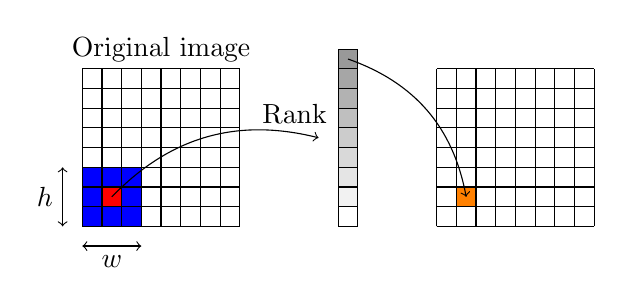
\begin{tikzpicture}[scale=0.25]
                \draw [fill=blue] (0, 0) rectangle (3, 3);
                \draw (0, 0) grid (8, 8);
                \draw (4, 9) node {Original image};
                \draw [fill=red] (1, 1) rectangle (2, 2);
                \draw [<->] (0, -1) -- (3, -1) node[below, pos=0.5] {$w$};
                \draw [<->] (-1, 0) -- (-1, 3) node[left, pos=0.5] {$h$};

                \foreach \i in {0,10,...,80}                    \draw [fill=gray!\i] (13, \i/10) rectangle (14, \i/10 + 1);

                \path[->] (1.5, 1.5) edge[bend left=30] node[above, pos=0.9] {Rank} (12, 4.5);

                \draw (18, 0) grid (26, 8);
                \draw [fill=orange] (19, 1) rectangle (20, 2);
                \path[->] (13.5, 8.5) edge[bend left=30] (19.5, 1.5);
            \end{tikzpicture}
        \end{column}
        \begin{column}{.5\textwidth}
            \begin{itemize}
                \item We decide on a window size $w \times h$ (other non-rectangular shapes are possible)
                \item We traverse each pixel in the image and take its $w \times h$ neighborhood
                \item We rank the intensity of each pixel in the neighborhood
                \item We take a specific value (e.g. minimum, maximum, mean, median) and set the output value to this value
            \end{itemize}
        \end{column}
    \end{columns}
\end{frame}

\begin{frame}
    {Example - median filter}
    \centering
    \includegraphics[width=.8\textwidth]{median_filter_example.png}
\end{frame}

\begin{frame}
    {Rank filters in Scikit Image}
    Rank filters are implemented in Scikit Image in the `skimage.rank` module.\\
    These filters require a \textit{footprint} of the pixel neighborhood, as a matrix of 0 and 1.

    For example

    \begin{codebox}
        \texttt{
            from skimage.rank import median\\
            \\
            \# 3x3 neighborhood\\
            footprint = np.ones(3, 3)\\
            img\_median = median(img, selem=footprint)
        }
    \end{codebox}
    \centering
    \includegraphics[width=.85\textwidth]{median_filter_different_footprints.png}
\end{frame}

\begin{frame}
    {Non-rectangular footprints}
    The footprint can be a \textit{non-rectangular} matrix. For example, you can generate a footprint with a \textbf{circular} shape using the \texttt{skimage.morphology.disk} function or one with a \textbf{diamond} shape using the \texttt{skimage.morphology.diamond} function.\\

    \vspace{2em}

    \begin{columns}
        \begin{column}{.5\textwidth}
            \begin{codebox}
                \texttt{from skimage.morphology import disk, diamond\\
                    \\
                    dsk = disk(7) \# A disk, radius 7\\
                    dia = diamond(7) \# A diamond, radius 7\\
                    \\
                    fig, ax = plt.subplots(1, 2)\\
                    ax[0].imshow(dsk, cmap="gray")\\
                    ax[1].imshow(dia, cmap="gray")
                }
            \end{codebox}
        \end{column}
        \begin{column}{.5\textwidth}
            \centering
            \includegraphics[width=\textwidth]{different_shaped_footprints.png}
        \end{column}
    \end{columns}
\end{frame}

\begin{frame}
    {Rank filters - use cases}
    Rank filters are very simple, but have useful applications.\\

    The \textbf{median and mean filter} are used to remove noise and to smooth images.\\
    \pause
    \vspace{1em}
    The \textbf{maximum filter} can be used in binary images to remove  small "holes". It is also a very common filter used in modern neural networks for image analysis.\\
    \only<2>{
        \centering
        \begin{figure}
            \includegraphics[width=.55\textwidth]{maximum_filter.png}
            \caption{\small{\color{gray}{The maximum filter can remove small holes in binary masks}\color{black}}}
        \end{figure}
    }
    \only<3>{
        \begin{flushleft}
            The \textbf{minimum filter} can be used to remove small bright spots.            
        \end{flushleft}
        \centering
        \begin{figure}
            \includegraphics[width=.55\textwidth]{minimum_filter.png}
            \caption{\small{\color{gray}{The minimum filter can remove small bright spots in binary masks}\color{black}}}
        \end{figure}
    }

\end{frame}
\end{document}

